\documentclass{article}

% packages and stuff
\usepackage[utf8]{inputenc}
\usepackage[headheight = 18pt, footskip = 10pt]{geometry}
    \geometry{a4paper}
    \geometry{left=0.5in, right=0.5in, top=.95in, bottom=.95in}
\usepackage{graphicx}
\usepackage{amsmath}
%Better boxed command in math mode
\usepackage{empheq}
%Input text files and code
\usepackage{verbatim}
%Bold math
\usepackage{bm}
%Cancel to in math mode
\usepackage{cancel}
% Input standalone tex documents
\usepackage{standalone}
\usepackage{subcaption}
\usepackage{ulem}
\usepackage{bigstrut}
\usepackage{bm}
\usepackage{multirow}
\usepackage{calc}
\usepackage{xkeyval}
\usepackage{color, soul}
\usepackage{ifthen}
\usepackage{import}
\usepackage{times}
\usepackage{longtable}
\usepackage{tabularx}
\usepackage{multicol}
\usepackage{wrapfig}
\usepackage[font={small,it}]{caption}
\usepackage[version=4]{mhchem}
\usepackage{booktabs}
\usepackage{longtable}
\usepackage{epigraph}

%New colors defined below
\definecolor{codegreen}{rgb}{0,0.6,0}
\definecolor{codegray}{rgb}{0.5,0.5,0.5}
\definecolor{codepurple}{rgb}{0.58,0,0.82}
\definecolor{backcolour}{rgb}{0.95,0.95,0.92}

% Include external pdf documents
\usepackage{pdfpages}

%Nice captions in floating figures
\usepackage{caption}

%%%%%%%%%%%%%%%%%%%%%%%%%%%%%%%%%%%%%%%%%%%%%%%%%%%%%%%%%%%%%%%%%%%%%%%%%%%%%%%%
\usepackage{fancyvrb}
\usepackage{comment}
\usepackage{enumerate}
\usepackage{subfiles}

%%%%%%%%%%%%%%%%%%%%%%%%%%%%%%%%%%%%%%%%%%%%%%%%%%%%%%%%%%%%%%%%%%%%%%%%%%%%%%%

% capital H is a champion
\usepackage{float}
    \restylefloat{table}

% make section styles non-lame
\usepackage{sectsty}
    \allsectionsfont{\mdseries\upshape}

% easy coloring for todo notes
\newcommand{\done}{\todo[inline, color=green]{(DONE)}{}}
\newcommand{\notdone}{\todo[inline, color=red]{(NOT DONE)}{}}
\newcommand{\fix}[1]{\todo[inline, color=red!75]{(FIX) #1}{}}
\newcommand{\discuss}[1]{\todo[inline, color=blue!40]{(DISCUSS) #1}{}}
\newcommand{\note}[1]{\todo[inline, color=yellow!20]{(NOTE) #1}}
\newcommand{\review}{\todo[inline, color=red!45!yellow!45]{(REVIEW)}{}}


\pagenumbering{gobble}
\setlength\parindent{10pt}
\setlength{\parskip}{0pt}
\setlength{\abovedisplayskip}{0pt}
\setlength{\belowdisplayskip}{0pt}
\relpenalty=10000 % don't split equations!!
\binoppenalty=10000 % don't split equations!!

\newcommand{\FigSiz}{0.37\textwidth}

% Set global figure size variable

\makeatletter
\define@key{Gin}{figsize}[true]{%
    \edef\@tempa{{Gin}{width=\FigSiz}}%
    \expandafter\setkeys\@tempa
}
\makeatother


%%%%%%%%%%%%%%%%%%%%%%%%%%%%%%%%%%%%%%%%%%%%%%%%%%%%%%%%%%%%%%%%%%%%%%%%%%%%%%%%%%%%%%%%%%%%%%%


% Custom title
\pagenumbering{arabic}
\usepackage{lastpage}
\usepackage{fancyhdr}
    \fancyhead{}
    \fancyfoot{}
    \pagestyle{fancy}
    \chead{\Large CS575: Project 4}
    \lhead{\Large Andrew Alferman}
    \rhead{\Large \today}
    \cfoot{\thepage  ~\ of ~\pageref{LastPage}}

\usepackage{titlesec}
\titlespacing*{\subsection}
{0pt}{0.65\baselineskip}{0.65\baselineskip}

%%%%%%%%%%%%%%%%%%%%%%%%%%%%%%%%%%%%%%%%%%%%%%%%%%%%%%%%%%%%%%%%%%%%%%%%%%%%%%%%%%%%%%%%%%%%%%%
\begin{document}



% Brief summary of the assignment
\begin{wrapfigure}{L}{0.25\textwidth}
        \begin{center}
        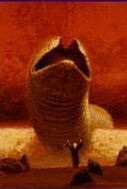
\includegraphics[width=0.17\textwidth]{Sandworm_heretics.jpg}
        \end{center}
        \caption{A sandworm.  Human shown in foreground for scale.}
        \label{fig:Sandworm}
\end{wrapfigure}
The purpose of this assignment was to adjust a simulation of the number of grain vs. the number of deer in a field by adding in parallel sections that run independently and adjust the state of the simulation.

Modifications to the original simulation included an increase in the number of deer to start out (\texttt{NowNumDeer} = 20), with a corresponding increase in the grain height (\texttt{NowHeight} = 30).  The reason for this is that the deer need a population of some size in order to sustain growth.  As one deer cannot reproduce by itself, a minimum of 2 deer are required to increase the population further.  The increase in the number of deer would eventually reach an equilibrium at a lower number of deer provided the same rate of grain consumption and growth, therefore to correct for these higher numbers, the amount of grain that one deer eats per month (\texttt{ONE\_DEER\_EATS\_PER\_MONTH}) was reduced to 0.1 inch, which may correspond to a selection of a larger field because each deer would eat a smaller average height of grain across that area.

In addition to modifying these initial parameters, the average rainfall per month (\texttt{AVG\_PRECIP\_PER\_MONTH}) and the average temperature (\texttt{AVG\_TEMP}) were made to be \texttt{float} instead of \texttt{constant float} for reasons that will soon become clear.  Finally, logic was added to ensure that the number of deer and the height of the grain could not ever be less than zero.

\subsection*{Question 1}
\textit{What was your own-choice quantity and how does it fit into the simulation.}

The quantity introduced into the simulation were sandworms inspired by the \textit{Dune} series of novels (see Figure \ref{fig:Sandworm}).  These enormous, ancient creatures are able to devour dozens of helpless deer at once in its gaping mouth.  Sandworms do not have eyes, but they are very sensitive to noise, particularly the rhythmic noise that creatures naturally make while walking normally.  This is a natural adaptation because their natural habitat is deep underground.  Occasionally, they breach the surface, consuming everything in their path, whether it be deer, grain, or rock.

Because of the large, indiscriminate nature of their feeding, each time a sandworm strikes it will consume large numbers of deer as well as a smaller quantity of grain.  Smaller populations of deer will flee in terror, spreading out so as to make less concentrated noise.  Because of this, the simulation is configured for the sandworms to eat fewer deer as the deer population (\texttt{NowNumDeer}) gets smaller.  The trigger for a sandworm attack is four of consecutive months of growth in deer population (tracked by \texttt{growthmos} in the code, which is assigned values by the \texttt{GrainDeer} function).  Large numbers of young deer are inexperienced in their dealings with sandworms, and so they will make lots of noise.  They must learn to walk without rhythm.  To ensure that the deer have a chance for survival, a sandworm will only occasionally feed, coming to the surface no sooner than every eight months (tracked by \texttt{monthswithoutstrike} in the \texttt{Sandworm} function of the code, initially starting at four months to allow the deer some time to get situated).  All changes to the number of deer are done by the \texttt{GrainDeer} function of the code, and the number of deer is tracked by the \texttt{tempDeer} and \texttt{NowNumDeer} variables, computed before the first \texttt{\#pragma omp barrier} statement.  The height of grain is changed by the \texttt{Grain} function in a similar manner, with the grain tracked by the \texttt{tempHeight} and \texttt{NowHeight} variables.

As a quirk of the life cycle of the sandworm, the amount of water available on the planet will steadily decrease (as seen by decreasing \texttt{tempprecip} and \texttt{AVG\_PRECIP\_PER\_MONTH} in the \texttt{Sandworm} function).  All this water will be brought deep underground by the larval stage of the sandworm, and there will be less precipitation.  Additionally, the average temperature of the planet will slowly increase (as seen by increasing \texttt{temptemp} and \texttt{AVG\_TEMP} in the \texttt{Sandworm} function).  Eventually, the planet will become a desert wasteland, void of all vegetation, but rich in a drug-like spice substance called melange that brings about clairvoyance and heightened awareness.  The deer must adapt by finding creative ways to conserve water and grow crops in isolated habitats. Though this may seem like an impossible task for the deer, they may stand a chance at survival if they choose to use the spice, which extends lifespan and heightens all abilities.  The melange has not yet been factored into the simulation.

All computations of the state variables are computed before the first \texttt{\#pragma omp barrier} statement, all variables are assigned new values before the second \texttt{\#pragma omp barrier} statement, and all printing and calculation of new temperature and precipitation occurs before the third \texttt{\#pragma omp barrier} statement.

\subsection*{Question 2}
\textit{Show a table for temperature, precipitation, number of deer, height of the grain, and your own-choice quantity as a function of month number.}

A table has been included in Table \ref{tab:Data} of Appendix \ref{app:Data}.

\newpage

\subsection*{Question 3}
\textit{Show a graph for temperature, precipitation, number of graindeer, height of the grain, and your own-choice quantity as a function of month number.}

\begin{wrapfigure}{r}{0.51\linewidth}
        \begin{center}
        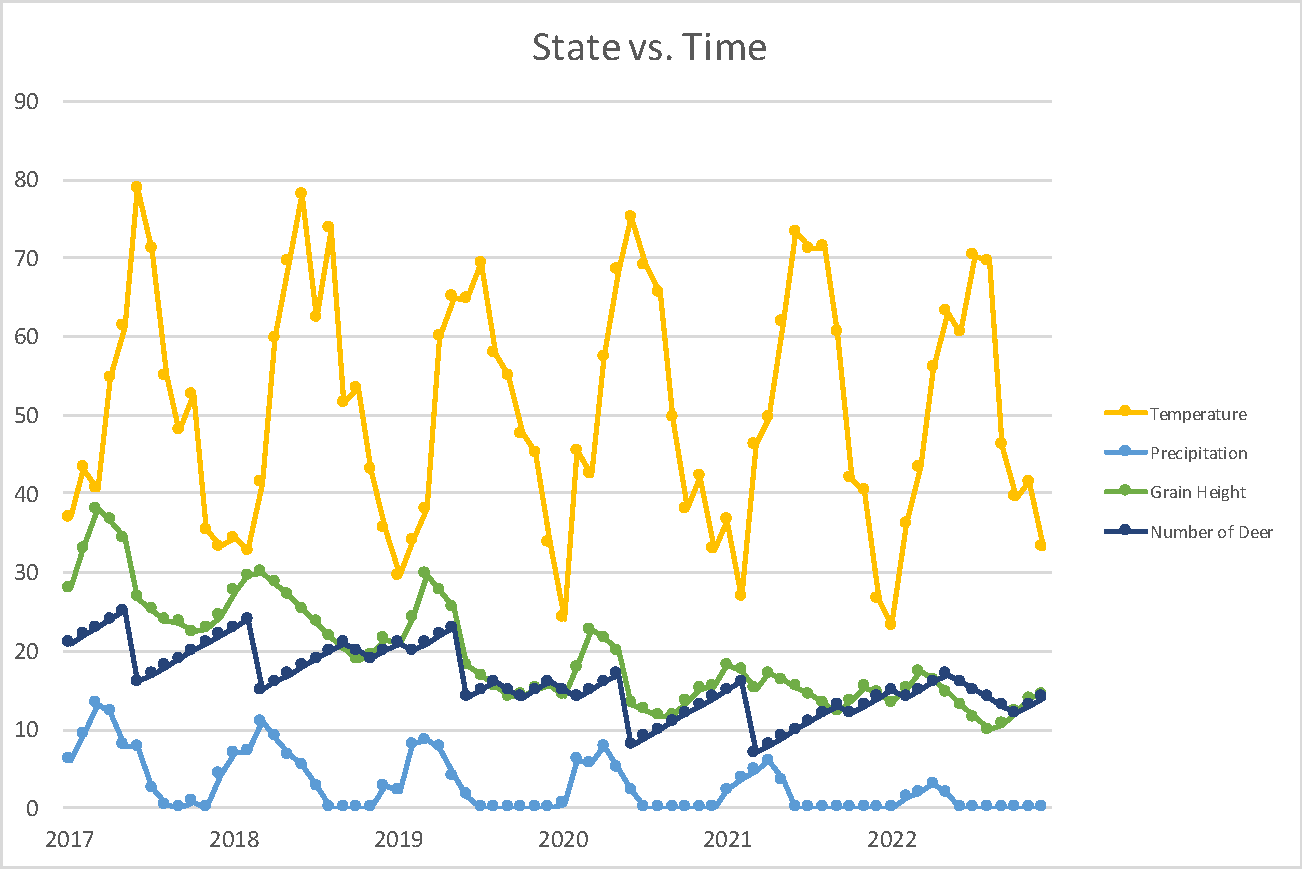
\includegraphics[width=1.0\linewidth]{Picture1.pdf}
        \end{center}
        \caption{State of the simulation over time.  Note the sharp declines in population that occur when sandworms strike.  As the population of deer get more experienced towards the end of the simulation, they learn to make less noise, attracting fewer sandworms.  Ultimately, however, they will be doomed unless they learn to conserve and reclaim water and grow crops in controlled environments.}
        \label{fig:State Plot}
\end{wrapfigure}

Figure \ref{fig:State Plot} plots all of the required information.  Note that the temperature is shown in $^\circ$C to provide better resolution in the graph.  No one knows exactly how many sandworms may exist.  The sandworms travel from afar, and their presence is not constant.  Because of this, the number of sandoworms has not been plotted.  However, their presence is made known in Figure \ref{fig:State Plot} by the sharp drops in population of deer, each of which correspond to a sandworm attack (the variable \texttt{Sandwormstrike} = 1 for that month, and resets to zero immediately afterwards, as determined by the \texttt{Sandworm} function).

\subsection*{Question 4}
\textit{Provide a commentary about the patterns in the graph and why they turned out that way.  What evidence in the curves proves that your own quantity is actually affecting the simulation?}

After sustained periods of growth in the deer population, the number of deer will sharply decline due to the sandworm attacks.  A smaller decrease in the average height of grain can also be seen when these attacks happen.  This indicates that the \texttt{Sandwormstrike} quantity is working as intended, causing the \texttt{GrainDeer} and \texttt{Grain} functions to adjust their numbers accordingly.  Additionally, the average precipitation steadily decreases over the course of the simulation, to the point where it is almost nothing by the end.  The average temperature also increases over the course of the simulation, however the trend is more difficult to see due to the large variation in temperature that occurs as part of the natural cycles, much like real life.  The increase in temperature and the decrease in precipitation causes the average height of grain in the simulation to decrease over time.  The decrease in grain has the effect of decreasing the number of deer as well, as seen by the small decrease in population of deer each month that the average height of the grain in inches is less than the number of deer.  If left to run much longer without interference, both the average grain height and the number of deer diminish towards zero, and the planet becomes a complete desert.

\newpage
\section{Appendices}
\subsection{Table of State Conditions by Month}
\label{app:Data}

\begin{longtable}{|l|l|l|l|l|l|}
\caption{Data Generated by Simulation}\label{tab:Data}\\
\hline
Month & Year & Temp  & Precip & Height & NumDeer \\ \hline
0     & 2017 & 31.88 & 5.74   & 28     & 21      \\ \hline
1     & 2017 & 45.05 & 10.75  & 32.07  & 22      \\ \hline
2     & 2017 & 42.81 & 12.93  & 36.65  & 23      \\ \hline
3     & 2017 & 62.05 & 11.39  & 34.41  & 24      \\ \hline
4     & 2017 & 67.41 & 10.31  & 32.01  & 25      \\ \hline
5     & 2017 & 77.58 & 5.64   & 29.51  & 26      \\ \hline
6     & 2017 & 70.69 & 2.15   & 21.91  & 17      \\ \hline
7     & 2017 & 55.87 & 0.06   & 20.45  & 18      \\ \hline
8     & 2017 & 61.02 & 0      & 18.69  & 19      \\ \hline
9     & 2017 & 45.37 & 0      & 19     & 18      \\ \hline
10    & 2017 & 44.87 & 0.8    & 19.91  & 19      \\ \hline
11    & 2017 & 39.93 & 4.58   & 23.97  & 20      \\ \hline
0     & 2018 & 35.39 & 4.9    & 26.95  & 21      \\ \hline
1     & 2018 & 40.41 & 9.86   & 32.84  & 22      \\ \hline
2     & 2018 & 38.84 & 9.65   & 38.52  & 23      \\ \hline
3     & 2018 & 57.03 & 10.55  & 36.66  & 24      \\ \hline
4     & 2018 & 58.95 & 9.54   & 29.48  & 15      \\ \hline
5     & 2018 & 71.97 & 5.92   & 27.98  & 16      \\ \hline
6     & 2018 & 78.04 & 1.26   & 26.38  & 17      \\ \hline
7     & 2018 & 59.29 & 0.22   & 24.76  & 18      \\ \hline
8     & 2018 & 49.32 & 0      & 24.19  & 19      \\ \hline
9     & 2018 & 39.34 & 0      & 25.22  & 20      \\ \hline
10    & 2018 & 34.38 & 0      & 25.37  & 21      \\ \hline
11    & 2018 & 27.2  & 0      & 23.84  & 22      \\ \hline
0     & 2019 & 40.81 & 2.43   & 26.12  & 23      \\ \hline
1     & 2019 & 38.73 & 7.51   & 31.22  & 24      \\ \hline
2     & 2019 & 41.11 & 9.5    & 31.7   & 15      \\ \hline
3     & 2019 & 52.27 & 8.55   & 31.94  & 16      \\ \hline
4     & 2019 & 61.67 & 7.76   & 30.41  & 17      \\ \hline
5     & 2019 & 75.14 & 2.51   & 28.71  & 18      \\ \hline
6     & 2019 & 74.08 & 0.2    & 26.91  & 19      \\ \hline
7     & 2019 & 65.18 & 0      & 25.02  & 20      \\ \hline
8     & 2019 & 57.69 & 0      & 23.15  & 21      \\ \hline
9     & 2019 & 45.48 & 0      & 23.23  & 22      \\ \hline
10    & 2019 & 33.47 & 0      & 22.95  & 23      \\ \hline
11    & 2019 & 31.29 & 0.49   & 22.17  & 22      \\ \hline
0     & 2020 & 37.62 & 3.13   & 24.68  & 23      \\ \hline
1     & 2020 & 40.56 & 6.05   & 29.2   & 24      \\ \hline
2     & 2020 & 40.8  & 4.99   & 32.99  & 25      \\ \hline
3     & 2020 & 52.38 & 6.9    & 32.06  & 26      \\ \hline
4     & 2020 & 61.04 & 5.34   & 29.54  & 27      \\ \hline
5     & 2020 & 76.75 & 2.36   & 21.84  & 18      \\ \hline
6     & 2020 & 67.96 & 0      & 20.04  & 19      \\ \hline
7     & 2020 & 64.2  & 0      & 18.15  & 20      \\ \hline
8     & 2020 & 51.78 & 0      & 16.88  & 19      \\ \hline
9     & 2020 & 45.77 & 0      & 17.09  & 18      \\ \hline
10    & 2020 & 42.76 & 0      & 18.02  & 17      \\ \hline
11    & 2020 & 41.32 & 0      & 19.21  & 18      \\ \hline
0     & 2021 & 39.51 & 0      & 20.34  & 19      \\ \hline
1     & 2021 & 52.78 & 2.04   & 19.27  & 20      \\ \hline
2     & 2021 & 53.37 & 5.28   & 18.34  & 19      \\ \hline
3     & 2021 & 59.04 & 5.47   & 16.62  & 18      \\ \hline
4     & 2021 & 76.38 & 0.54   & 14.82  & 17      \\ \hline
5     & 2021 & 76.05 & 0.3    & 13.12  & 16      \\ \hline
6     & 2021 & 69.39 & 0      & 11.52  & 15      \\ \hline
7     & 2021 & 73.05 & 0      & 10.02  & 14      \\ \hline
8     & 2021 & 54.12 & 0      & 9.02   & 13      \\ \hline
9     & 2021 & 60.28 & 0      & 7.77   & 12      \\ \hline
10    & 2021 & 35.99 & 0      & 9.07   & 11      \\ \hline
11    & 2021 & 44.13 & 0      & 10.45  & 10      \\ \hline
0     & 2022 & 38.69 & 0      & 12.35  & 11      \\ \hline
1     & 2022 & 35.61 & 1.77   & 14.6   & 12      \\ \hline
2     & 2022 & 63.51 & 3.83   & 13.42  & 13      \\ \hline
3     & 2022 & 64.75 & 1.34   & 12.13  & 14      \\ \hline
4     & 2022 & 73.14 & 0      & 10.73  & 13      \\ \hline
5     & 2022 & 80.11 & 0      & 4.43   & 9       \\ \hline
6     & 2022 & 72.55 & 0      & 3.53   & 8       \\ \hline
7     & 2022 & 66.98 & 0      & 2.73   & 7       \\ \hline
8     & 2022 & 69.02 & 0      & 2.03   & 6       \\ \hline
9     & 2022 & 52.91 & 0      & 1.98   & 5       \\ \hline
10    & 2022 & 40.82 & 0      & 4.41   & 4       \\ \hline
11    & 2022 & 32.79 & 0      & 5.76   & 5       \\ \hline
\end{longtable}

\end{document}
